\section{Apprendimento non supervisionato}
\label{app_non_sup}

Nel capitolo precedente è stata mostrata l'utilità degli algoritmi di apprendimento supervisionato, osservando che, nel caso in cui si abbiano a disposizione sia i vettori di input che i corrispettivi output target, si può ottenere un'approssimazione della relazione esistente input-output.
Tuttavia non è sempre possibile avere a disposizione gli output target e bisogna capire se è comunque possibile ottenere informazioni utili dai dati. \\
Come già accennato nelle prime pagine di questa trattazione quando non si hanno a disposizione gli output target si possono applicare tecniche di apprendimento non supervisionato, dove l'obiettivo è quello di trovare eventuali partizioni degli input (Clustering). \\
Si consideri la figura ~\ref{Unsup} dove sono riportate tre diverse configurazioni possibili nel caso di input bidimensionali: è evidente che nel caso a) sia possibile la separazione in due sotto gruppo e nel caso b) in un unico sotto gruppo, mentre nel caso c) sembrerebbe non si possano stabilire graficamente eventuali separazioni.

\begin{figure}[h!]
	\centering
	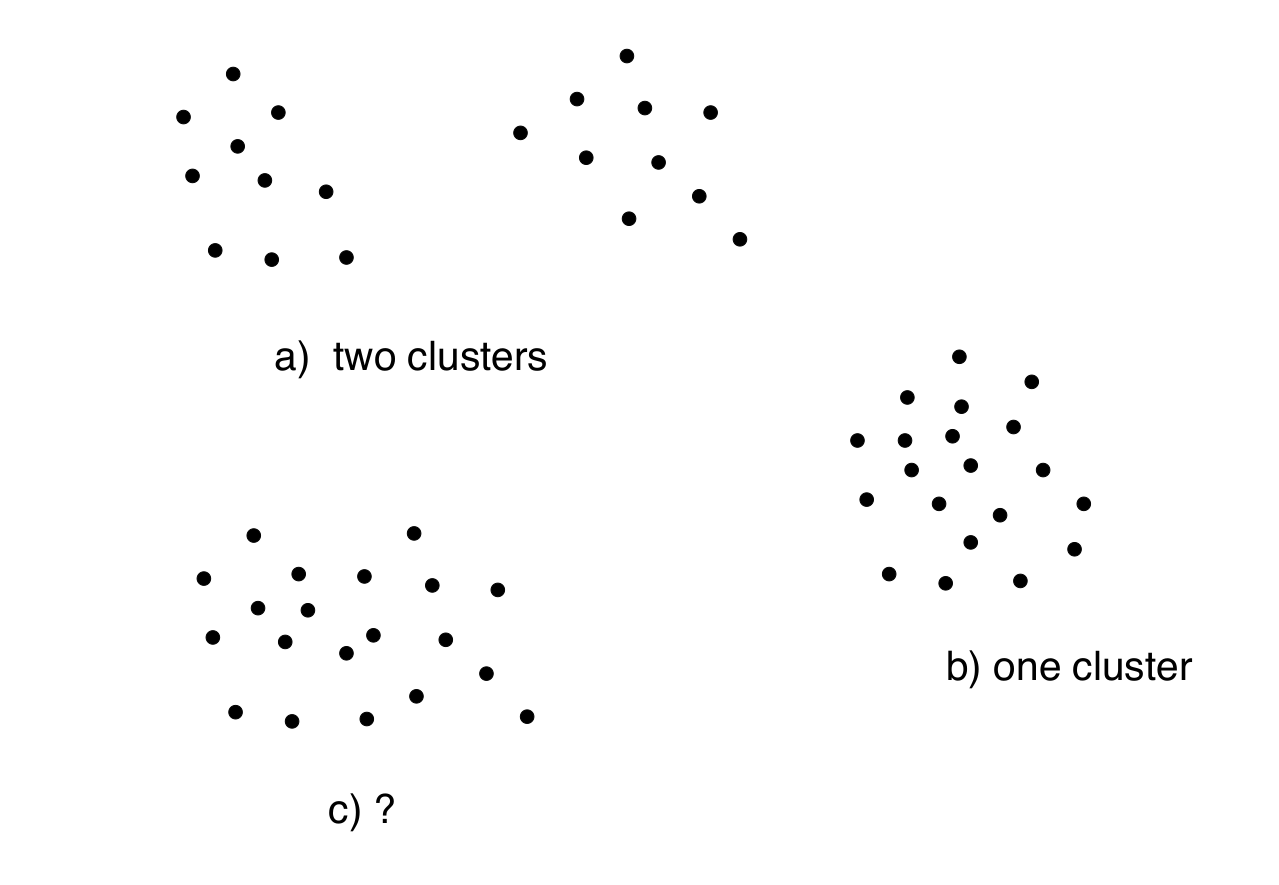
\includegraphics[width=0.85\textwidth]{figs/Unsup_learning.png}
	\caption{vettori di input in uno spazio bidimensionale in tre situazioni differenti. L'immagine è presa da \cite{IntroML}}
	\label{Unsup}
\end{figure}

Quindi un algoritmo di clustering si occupa della suddivisione del set di input $\Sigma$ in un numero N di sottogruppi $\Sigma_1$,...,$\Sigma_n$, detti appunto cluster; si noti che lo stesso numero N non viene stabilito a priori e fornito all'algoritmo, ma viene anch'esso ricavato a partire dai dati. Una volta fatto sarà possibile implementare un classificatore per collegare nuovi vettori di input con i cluster precedentemente individuati.\\
Inoltre, aumentando il livello di complessità, è possibile trovare eventuali gerarchie di partizionamento, ovvero cluster di cluster.

\newpage

\subsection{Metodologie di clustering}
\label{metodologie di clustering}
Si descrivono due diverse metodologie di clustering, di cui una basata sul concetto di distanza ed una su quello di probabilità.

\subsubsection{Metodo basato sulla distanza euclidea}
\label{metodo distanza euclidea}
Gli algoritmi di apprendimento non supervisionato sfruttano una qualche misura di similarità per separare i pattern (gli input) nei vari cluster. Una possibilità è quella di utilizzare la semplice distanza euclidea per poter separare lo spazio n-dimensionale dei pattern in delle sotto-aree, che sono appunto i cluster. \\
Per fare ciò viene implementato un metodo iterativo, basato sulla definizione di alcuni punti particolari nello spazio dei pattern, detti "cluster seekers" (letteralmente "cercatori di cluster"). \\
Si definiscono M punti nello spazio n-dimensionale $\textbf{C}_\textbf{1},...,\textbf{C}_\textbf{M}$ e l'obiettivo è quello di fare in modo che ogni punto si muova verso il centro di ogni singolo cluster, in modo che ogni cluster abbia al suo centro uno di questi cluster seekers. \\
Come è già stato spiegato precedentemente, l'algoritmo non conosce a prescindere il numero di cluster ma riesce a ricavarlo dai pattern stessi; per questa ragione il numero di cluster seekers M è inizialmente casuale ed esiste un procedura per ottimizzarlo, che verrà illustrata in seguito. \\
I pattern del training data set $\Sigma$ vengono presentati all'algoritmo uno alla volta: per ognuno di essi ($\textbf{x}_\textbf{i}$) si cerca il cluster seekers più vicino ($\textbf{C}_\textbf{k}$) e lo si sposta verso $\textbf{x}_\textbf{i}$ nel seguente modo:
\begin{equation}
\textbf{C}_\textbf{k} + \alpha_k(\textbf{x}_\textbf{i} - \textbf{C}_\textbf{k}) \rightarrow \textbf{C}_\textbf{k}
\end{equation}
dove $\alpha_k$ è un parametro di apprendimento che determina di quanto il cluster seeker k-esimo si muove verso il punto $\textbf{x}_\textbf{i}$


\newpage